\documentclass[11pt,a4paper]{article}
\usepackage[T1]{fontenc}
\usepackage[utf8]{inputenc}
\usepackage{lmodern,microtype}
\usepackage[margin=22mm,headheight=15pt]{geometry}
\usepackage{amsmath,amssymb,booktabs,tabularx,array,enumitem}
\usepackage{xcolor,graphicx}
\usepackage{tikz}
\usetikzlibrary{arrows.meta,positioning,shapes.geometric}
\usepackage{tcolorbox}
\tcbuselibrary{breakable}
\usepackage{fancyhdr,hyperref}
\definecolor{ink}{HTML}{18354A}
\definecolor{teal}{HTML}{087E8B}
\definecolor{pale}{HTML}{EDF5F6}
\definecolor{gold}{HTML}{AD6B20}
\hypersetup{colorlinks=true,linkcolor=teal,citecolor=teal,urlcolor=teal,pdftitle={Constructing an Agent-Based Model},pdfauthor={ABM course}}
\pagestyle{fancy}\fancyhf{}
\fancyhead[L]{\small\sffamily ABM\_course\quad /\quad Session 4}
\fancyhead[R]{\small\sffamily Construction and ontology}
\fancyfoot[L]{\footnotesize\sffamily Constructing an Agent-Based Model}
\fancyfoot[R]{\sffamily\thepage}
\renewcommand{\headrulewidth}{0.3pt}
\setlength{\emergencystretch}{2em}
\setlength{\parindent}{0pt}\setlength{\parskip}{6pt}
\setcounter{secnumdepth}{3}
\setcounter{tocdepth}{2}
\raggedbottom
\setlist{nosep,leftmargin=1.5em}
\newtcolorbox{principle}[1]{breakable,colback=pale,colframe=teal,boxrule=.6pt,arc=2pt,title={#1},fonttitle=\bfseries,top=5pt,bottom=5pt}
\newtcolorbox{soccer}[1]{colback=gold!5,colframe=gold!65,boxrule=.5pt,arc=2pt,title={Soccer laboratory: #1},fonttitle=\bfseries,top=5pt,bottom=5pt}
\newcommand{\stereo}[1]{\texttt{\guillemotleft #1\guillemotright}}
\newcommand{\stage}[1]{\textsf{\textbf{#1}}}
\newcolumntype{Y}{>{\raggedright\arraybackslash}X}
\tikzset{box/.style={draw=teal,fill=pale,rounded corners=2pt,align=center,font=\small,inner sep=7pt},arr/.style={-{Stealth[length=2mm]},thick,draw=ink}}

% Fit long display equations to the available width without altering their content.
\newsavebox{\displaybox}
\newenvironment{fitdisplay}{\par\medskip\noindent\begin{lrbox}{\displaybox}$\displaystyle}{% 
$\end{lrbox}\makebox[\linewidth][c]{\ifdim\wd\displaybox>\linewidth\resizebox{\linewidth}{!}{\usebox{\displaybox}}\else\usebox{\displaybox}\fi}\par\medskip}
\begin{document}
\thispagestyle{empty}
{\sffamily\color{teal}\large ABM\_course / Teaching guide / Session 4\par}
\vspace{7mm}
{\sffamily\bfseries\color{ink}\fontsize{28}{32}\selectfont Constructing an\\Agent-Based Model\par}
\vspace{4mm}
{\large From Organized Complexity to Prospective Claims and Actionability\par}
\vspace{5mm}

\section*{Purpose}

The central methodological problem is not simply how to program an ABM. It is:

\begin{fitdisplay}
\boxed{\textbf{How do we decide what ABM to construct?}}
\end{fitdisplay}

Once the model exists, a second problem follows:

\begin{fitdisplay}
\boxed{\textbf{What can we defensibly claim from it?}}
\end{fitdisplay}

The guide therefore moves from \textbf{ex-ante construction} to \textbf{ex-post accountability}:

\begin{fitdisplay}
\boxed{
\text{EX ANTE: CONSTRUCT}
\rightarrow
\text{SIMULATE}
\rightarrow
\text{EX POST: DOCUMENT \& ASSESS}
}
\end{fitdisplay}



\clearpage
\begin{principle}{Source boundaries and course terminology}
This session introduces six new readings that build on the foundations developed in earlier sessions, including Simon \cite{simon_behavioral_1955,simon}, Weaver \cite{weaver}, Axtell \cite{axtell_why_2000-1}, Macy--Willer \cite{macy_factors_2002}, and Kollman--Page \cite{kollman_chapter_2006}. The guide brings those earlier foundations into conversation with the new readings to address ABM construction. Citations distinguish reading-grounded contributions from this course's synthesis. ``Bottom-up + along the way,'' the Four As, the parsimonious I-ABM heuristic and the distinction between $A_{3m}$ and $A_{3s}$, auditability/actionability, and the broad use of ``meta-analysis'' are course conventions. The six-class relational grammar, situated-agency triad, and practice-transition notation introduced below are also course synthesis. They are not attributed as a combined framework to the readings.

Ex ante and ex post distinguish methodological questions. Documentation can begin during construction, and later assessment can prompt revision.
\end{principle}
\clearpage
\tableofcontents
\clearpage
\section{From Previous Sessions: Foundations for Studying Complex Systems}
\label{sec:previous-foundations}

Session 4 builds on the earlier readings. Their contributions establish why organization, agency, and interaction matter, and why agent-based computation can be useful for studying them.

\begin{description}[style=nextline,leftmargin=0pt,itemsep=6pt]
\item[Weaver --- Organized complexity]
Weaver distinguishes simplicity, disorganized complexity, and organized complexity. The latter directs attention to interdependent factors whose organization matters to the phenomenon \cite{weaver}.

\item[Simon --- Decision-making and the architecture of complexity]
Simon's behavioral account of rational choice brings information and computational limits into the representation of decision-making \cite{simon_behavioral_1955}. His account of hierarchy and near-decomposability highlights subsystems and the differences between interactions within and between them \cite{simon}. Together, these readings draw attention to both decision processes and system organization.

\item[Axtell --- Why use agents?]
Axtell distinguishes uses of agent computation according to its relationship with mathematical formulations: presenting or computing solutions, exploring models that cannot be fully solved, and systematically investigating processes for which an equation-based formulation is not useful \cite{axtell_why_2000-1}. The reason for choosing ABM therefore depends on the problem being investigated.

\item[Macy--Willer --- From factors to actors]
Macy and Willer examine social processes through interacting adaptive agents and show how local interactions can generate aggregate patterns. Their review emphasizes relational microfoundations, networks that shape and are shaped by interaction, and computational experiments \cite{macy_factors_2002}.

\item[Kollman--Page --- Computational models of politics]
Kollman and Page connect computational modeling to political questions, including collective action, institutional design and performance, and electoral competition. Their discussion highlights adaptation, differences among agents, externalities, path dependence, geography, networks, and emergence \cite{kollman_chapter_2006}.
\end{description}

\begin{principle}{The transition to Session 4}
These earlier contributions motivate attention to organized complexity, bounded decision-making, interaction, and computational inquiry. The course now turns to a construction question: \textbf{How do we decide what ABM to build?} The following heuristics organize our response; they are course synthesis rather than a shared framework proposed by the earlier authors.
\end{principle}

\clearpage
\section{Foundations: Thinking About ABM Construction}

Building on those earlier foundations, two heuristics organize ABM construction in Session 4:

\begin{fitdisplay}
\boxed{\textbf{BOTTOM-UP}}
\qquad+\qquad
\boxed{\textbf{ALONG THE WAY}}
\end{fitdisplay}

These are \textbf{not opposites}.

\begin{itemize}
\item \textbf{Bottom-up} organizes a generative spiral of model construction and revision.
\item \textbf{Along the way} identifies additional questions that arise as the model is progressively constructed.
\end{itemize}

\subsection{Bottom-Up: The Generative Spiral}

The \textbf{generative spiral} is a course synthesis: Epstein supplies the generative question, while Cioffi-Revilla supplies progressive model construction inspired by Lakatos \cite{epstein,cioffi}. The spiral describes returning to construction with a revised specification; progress need not mean adding detail.

\subsubsection{Epstein --- Generate}

Epstein asks how a micro-specification can generate a macro-regularity \cite[pp.~41--43]{epstein}. Generation provides a candidate explanation; it does not uniquely identify the real mechanism. The generative question is:

\begin{quote}
\textbf{How could local interactions among heterogeneous autonomous agents generate the macro-pattern of interest?}
\end{quote}

\begin{fitdisplay}
\boxed{
\text{Micro-specification}
\rightarrow
\text{Interaction}
\rightarrow
\text{Macro-pattern}
}
\end{fitdisplay}

The modeller constructs the model, not its emergent outcome:

\begin{fitdisplay}
\boxed{
\text{CONSTRUCT THE MODEL}
\neq
\text{CONSTRUCT THE OUTCOME}
}
\end{fitdisplay}

Therefore:

\begin{fitdisplay}
\boxed{\textbf{Construct the conditions of possibility, not the emergent result.}}
\end{fitdisplay}

\subsubsection{Cioffi-Revilla --- Construct Progressively}

Cioffi-Revilla motivates theoretically guided model sequences with inspiration from Lakatos \cite{cioffi}. The course develops this into explicit ontological re-specification, including removal and reclassification. Begin with a deliberately restricted model and progressively re-specify it:

\begin{fitdisplay}
\boxed{
O_0\rightarrow O_1\rightarrow O_2\rightarrow\cdots
}
\end{fitdisplay}

Progressive construction is \textbf{not}:

\begin{fitdisplay}
O_{n+1}=O_n+\text{more detail}
\end{fitdisplay}

Instead:

\begin{fitdisplay}
\boxed{
O_{n+1}=\operatorname{re-specify}(O_n)
}
\end{fitdisplay}

using operations such as:

\begin{fitdisplay}
\boxed{
\text{ADD}
\quad
\text{REMOVE}
\quad
\text{DE-/RECLASSIFY}
\quad
\text{RECOMBINE}
}
\end{fitdisplay}

These operations have the following meanings in the course's construction vocabulary:

\begin{description}[style=nextline,leftmargin=0pt,itemsep=4pt]
\item[ADD] Introduce an element, attribute, capability, or relation previously absent from the specification because the question now requires it.
\item[REMOVE] Eliminate a represented element or distinction that is unnecessary, redundant, or no longer justified for the question.
\item[DE-/RECLASSIFY] Revise existing categories or modeling roles---for example, split one category into two, merge two categories, or change an element from one type to another.
\item[RECOMBINE] Reorganize how represented elements are connected or grouped, changing the configuration of the system.
\end{description}

A revision may combine several operations; each should be justified by the modeling question.

Thus:

\begin{fitdisplay}
\boxed{
\textbf{Progressive construction}
=
\textbf{progressive ontological re-specification}
}
\end{fitdisplay}



\subsection{Along the Way: Balancing Parsimony and Context}

Parsimony keeps representation focused on the modeling question. Along the way, contextual requirements can reveal which initial simplifications need revision. We consider institutional structuring through Ghorbani/Ostrom, situated agency through Knoeri/Giddens, and then social recursivity. These complementary contributions help us reconsider what is minimally sufficient for the question.

\subsubsection{Ghorbani / Ostrom --- Institutionally Structured Agency}

When institutional prescriptions matter to the question, the usefulness of the model depends on representing their actual role in action. Listing the rules is insufficient: we need to specify how agents respond to them. Ask:

\begin{quote}
\textbf{How do institutional prescriptions influence what agents actually do?}
\end{quote}

Institutions structure action possibilities without mechanically determining behavior:

\begin{fitdisplay}
\boxed{
\text{Institution}
\rightarrow
\text{Structured possibilities}
\rightarrow
\text{Agent decision}
\rightarrow
\text{Action}
}
\end{fitdisplay}

Ghorbani et al., building on Ostrom's institutional analysis, discuss how institutions structure action and how agents respond to institutional prescriptions \cite{ghorbani}. We draw on this contribution to examine institutions and their enactment: what is prescribed and what agents actually do. \footnote{MAIA (Modelling Agent systems based on Institutional Analysis) is Ghorbani et al.'s framework, developed from Ostrom's IAD (Institutional Analysis and Development). They provide the background to the reading's treatment of institutions \cite{ghorbani}.}

\begin{principle}{From institutional prescriptions to rules in use}
Ostrom's emphasis on the rules actually used to organize recurring interaction, as presented by Ghorbani et al., directs attention to how institutions operate in practice \cite[sec.~2.3]{ghorbani}. Identifying a prescription is therefore a starting point: how does it enter agents' decisions and the interactions that follow?

Ghorbani et al. explicitly allow agents to disregard institutions under certain conditions \cite[sec.~2.4]{ghorbani}. An obligation specifies what an agent should do; it does not guarantee compliance. If compliance varies in reality, making every agent follow every prescription removes a potentially important source of variation and limits the model's ability to explain how institutions operate in practice.
\end{principle}

The modeling task is therefore to represent how agents respond to prescriptions. Their commitment to institutional goals, immediate needs, and expected sanctions may influence compliance; which factors to include depends on the question.

For example, agents asked to limit their use of a shared resource may comply out of commitment to conservation or fear of sanctions, while others exceed the limit to meet immediate needs. This course illustration shows why prescribing a limit and modeling its effects are different tasks.

As agents encounter institutions---through acceptance, habit, or coercion---their expectations and ways of acting may change. How can we represent agents whose decisions are shaped by these conditions, and whose actions may, in turn, reproduce or transform them?

\subsubsection{Knoeri / Giddens --- Situate Agency}

\begin{fitdisplay}
\boxed{\textbf{Agency is situated.}}
\end{fitdisplay}

The parsimony maintained so far may now require a substantial revision: the question may demand agents whose decisions are sensitive to their context. Knoeri et al. provide an approach to operationalizing context-specific agents, interactions, decisions, and behavior, drawing on Giddens and empirical knowledge of the system \cite{knoeri}.

Context extends beyond other agents. It includes the environment in which action occurs and the artifacts and institutional conditions that enable, constrain, or mediate it. In the course vocabulary, we distinguish two forms of \textbf{Artificiality}:

\begin{description}[style=nextline,leftmargin=0pt,itemsep=4pt]
\item[Material Artificiality] Tools, technologies, infrastructure, and other artifacts that shape what agents can do.
\item[Social Artificiality] Rules, norms, roles, and authority arrangements that shape what agents are expected, permitted, or forbidden to do.
\end{description}

Representing these conditions is only part of the task. We also need to specify how agents perceive and respond to them. A situated agent's decisions depend on its access to material means and its interpretation of social expectations, alongside its own needs and capabilities.

The further construction challenge is to represent agents \textbf{dynamically endogenizing the influence of Artificiality}: experience with tools, rules, and institutions may enter their evolving expectations, habits, and decision processes. For example, repeated use of a tool may change how an agent performs a task; experience with a rule may change its willingness to comply. These are course illustrations of mechanisms to specify when the question requires them, rather than automatic consequences of adding context to the model.

This leads to a further question: how do agents' actions, in turn, reproduce or transform the material and social conditions of subsequent action?

\subsubsection{Giddens --- Social Recursivity}

Through Knoeri et al.'s use of Giddens, we encounter a further idea: agents draw on existing rules and resources when they act, and their practices help reproduce or transform those same conditions \cite{knoeri}. Social structure is therefore both a condition of action and something sustained or changed through action. This is the sense of \textbf{social recursivity} developed here.

\begin{principle}{Recursivity through practice}
People act under conditions inherited from earlier interactions. In using, interpreting, following, or contesting those conditions, they contribute to the conditions of subsequent action. Repetition may sustain an established practice; it may also modify that practice, deliberately or unintentionally.
\end{principle}

A mathematical comparison helps clarify the idea. In the Fibonacci recurrence,
\begin{fitdisplay}
F_{n+1}=F_n+F_{n-1},\qquad F_0=0,\quad F_1=1,
\end{fitdisplay}
the rule and initial values determine each subsequent value. The numbers do not interpret or contest the rule. Social recursivity is less straightforward: people interpret expectations, respond to others, and act with unequal resources and authority. Their actions may sustain or alter the rules and relations organizing their interaction. The comparison is a course illustration, not a claim that Giddens proposes a mathematical recurrence.

For example, people joining a queue encounter an expectation about whose turn comes next. By waiting and recognizing others' turns, they help sustain that convention. If some claim priority and others accept or challenge the claim, the practice may be reinforced, modified, or disputed. The conditions of the next interaction depend partly on what people have just done.

\begin{center}
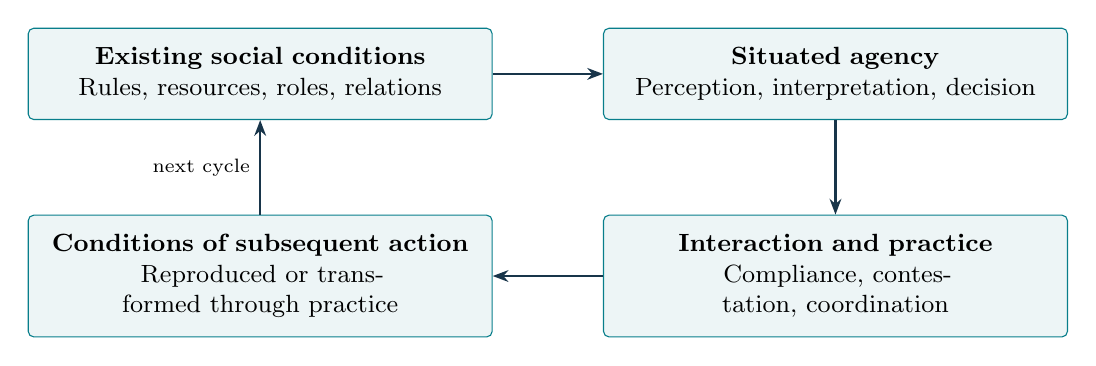
\begin{tikzpicture}[node distance=12mm and 14mm]
\node[box,text width=5.4cm] (s) {\textbf{Existing social conditions}\\Rules, resources, roles, relations};
\node[box,text width=5.4cm,right=of s] (a) {\textbf{Situated agency}\\Perception, interpretation, decision};
\node[box,text width=5.4cm,below=of a] (i) {\textbf{Interaction and practice}\\Compliance, contestation, coordination};
\node[box,text width=5.4cm,below=of s] (n) {\textbf{Conditions of subsequent action}\\Reproduced or transformed through practice};
\draw[arr] (s)--(a);\draw[arr] (a)--(i);\draw[arr] (i)--(n);
\draw[arr] (n)--node[left,font=\scriptsize,align=right]{next cycle}(s);
\end{tikzpicture}
\end{center}
{\small\textbf{Figure 1. Social recursivity through practice (course synthesis).} Arrows show conditioning and the continuation of practice. The next cycle begins under the resulting conditions, which may persist or change. The diagram separates moments for explanation; in social life, these processes may overlap.}

Recursivity does not require constant change: maintaining a convention also depends on its continued enactment. Nor does recursivity alone establish chaos or unpredictability. An ABM can represent these processes with explicitly specified mechanisms, including deterministic ones; the modeling task is to decide how agents' actions sustain or alter the conditions relevant to the question.

A useful \textbf{course synthesis, not a direct quotation}, is:
\begin{fitdisplay}
\boxed{\textbf{History conditions action; practice sustains or transforms its conditions.}}
\end{fitdisplay}

This also provides a course bridge to Simon: organization helps us understand persistence, while Giddens directs attention to the practices through which social organization is reproduced or transformed.

\subsection{Bottom-Up + Along the Way}

The generative spiral proceeds through successive model specifications:

\begin{fitdisplay}
\boxed{
O_0
\longrightarrow
O_1
\longrightarrow
O_2
\longrightarrow
O_n
}
\end{fitdisplay}

But along that trajectory:

\begin{fitdisplay}
\boxed{
\begin{array}{ccccccc}
O_0 &\longrightarrow& O_1 &\longrightarrow& O_2 &\longrightarrow& O_n\\
&&\uparrow&&\uparrow&&\uparrow\\
&&\text{articulate}&&\text{situate}&&\text{empirically}\\
&&\text{institutions}&&\text{agency}&&\text{ground}
\end{array}}
\end{fitdisplay}

The heuristic is:

\begin{fitdisplay}
\boxed{
\textbf{Start generatively. Construct progressively.}
\atop
\textbf{Along the way, situate the model where the question requires it.}
}
\end{fitdisplay}

These interventions can recur at any revision; they are not compulsory stages. A richer model can remain generative.



\clearpage
\section{Ex Ante: Constructing the Ontology}

The ex-ante question is:

\begin{fitdisplay}
\boxed{\textbf{What are we going to model?}}
\end{fitdisplay}

The construction heuristic is:

\begin{fitdisplay}
\boxed{
\textbf{DISSECT}
\rightarrow
\textbf{DISCRETIZE}
\rightarrow
\textbf{COMBINE}
}
\end{fitdisplay}



\subsection{Dissect}

Start from the phenomenon:

\begin{fitdisplay}
\text{Phenomenon}
\xrightarrow{\text{dissect}}
\text{Relevant distinctions}
\end{fitdisplay}

\textbf{Question:}

\begin{quote}
What distinctions are necessary for investigating the phenomenon?
\end{quote}

Dissection is analytical.



\subsection{Discretize}

Decide which distinctions become explicit modeled elements.

The first three As provide the basic vocabulary:

\begin{fitdisplay}
\boxed{A_1,\;A_2,\;A_3}
\end{fitdisplay}

\subsubsection{\(A_1\) --- Agent}

\begin{quote}
\textbf{An entity whose endogenous agency is necessary for the explanatory or decision problem.}
\end{quote}

\textbf{Question:}

\begin{fitdisplay}
\boxed{\text{Who has endogenous agency?}}
\end{fitdisplay}

\subsubsection{\(A_2\) --- Arena}

\begin{quote}
\textbf{The material, spatial, ecological, or environmental substrate within which action occurs.}
\end{quote}

\textbf{Question:}

\begin{fitdisplay}
\boxed{\text{Where does action occur?}}
\end{fitdisplay}

\subsubsection{\(A_3\) --- Artificiality}

\begin{quote}
\textbf{Human-made artifacts and socially constructed institutions that mediate agents' relations with other elements of the modeled world.}
\end{quote}

Here, \textbf{artificial} means made or instituted through human activity rather than naturally occurring. It does not mean unreal: tools, infrastructure, rules, and institutions can have real effects on action. Artificiality enables, constrains, or redirects how agents interact with one another and with their environment.

\begin{fitdisplay}
\boxed{A_3=A_{3m}+A_{3s}}
\end{fitdisplay}
The plus sign denotes conceptual composition, not numerical addition.

\begin{description}[style=nextline,leftmargin=0pt]
\item[$A_{3m}$ --- Material Artificiality] Tools, technologies, infrastructure, and other human-made artifacts that mediate action. A traffic-light device can be represented here.
\item[$A_{3s}$ --- Social Artificiality] Institutions, norms, formal rules, roles, and authority arrangements. The obligation to stop at a red light and the authority to sanction violations can be represented here.
\end{description}

Including particular artifacts and institutions makes the model more contextualized: its account of action now depends on those arrangements. This narrows the conditions under which its results can be generalized without further justification. The added specificity should serve the modeling question.

\begin{principle}{Artificiality is not decorative}
Explicit Artificiality adds modeling complexity: its relevant properties, relations, and effects on action must be specified. Represent a traffic light when the intention is to investigate how it affects traffic. This requires specifying what agents perceive and how they respond to its signals, including compliance or non-compliance where relevant. Merely drawing a traffic light does not represent its mediation of action.
\end{principle}

%

A useful heuristic is:
\begin{fitdisplay}
\boxed{\text{Artificiality}=\text{affordance and/or barrier}}
\end{fitdisplay}

\subsection{Combine: \(A_4\) --- Array}

Discrete elements must be arranged into a system.

\begin{quote}
\textbf{Array is the assumed systemic arrangement organizing Agents, Arena and Artificiality.}
\end{quote}

\begin{fitdisplay}
\boxed{
A_4=\mathcal C(A_1,A_2,A_3)
}
\end{fitdisplay}

Here, $\mathcal C$ denotes configuration, not a transition rule. At a given time, $A_4(t)=\mathcal C(A_1(t),A_2(t),A_3(t))$ describes the arrangement then obtaining. A configuration can change during a run; the mechanism producing that change is specified separately in dynamics.

\textbf{COMBINE is an explicit modeling operation.} Listing elements and their capabilities does not yet connect them. COMBINE establishes the potential pathways through which methods can affect states of connected elements. A link need not be labeled: it provides a pathway, while each method specifies how it uses that pathway, under which conditions, and which states it may affect. A connection alone produces no effect. The following construction checks make that task concrete:

\begin{description}[style=nextline,leftmargin=0pt,itemsep=5pt]
\item[Provide a path for influence.] Without a represented path of influence, an element cannot affect or be affected by another. The path may be direct or mediated by other agents, artifacts, or the environment. An indirect connection through the environment must also be specified: one element's method changes an environmental state that another element's method can read or respond to. Mere co-location does not establish influence.

\item[Connect capabilities to their conditions of use.] A method may be correctly specified yet never be enacted because the agent lacks access to the information, resource, or counterpart it requires. A weak or unreliable connection may limit its enactment. For example, if the model includes drivers and traffic lights, a driver's method ``see the color'' requires a connection to the traffic light whose state it reads. The connection provides the pathway; the method specifies how the driver reads the color and under which conditions.

\item[Distinguish connectivity from the direction of effects.] An unlabeled link does not imply mutual effects. The methods using the pathway specify the direction of each effect and whether influence occurs both ways. A driver's perception method may read a signal's state without changing it; a sensor-controlled signal may also use information about approaching vehicles. Neither effect nor reciprocity follows from the line alone.

\item[Exclude genuine isolates.] An element may affect others without itself being affected. Its states may remain fixed, but a connection is still required for another element's method to read or use them. For example, an arena's fixed dimensions may constrain agents' movement. Immutability alone therefore does not make an element decorative. A genuine isolate has no actual or possible connection through which it affects or is affected by the modeled system. Such an element contributes nothing to the modeled interactions: specify the missing connection or remove the unnecessary element.
\end{description}

\begin{principle}{The modeler's judgment becomes especially visible in COMBINE}
Recognizing relevant elements is only part of understanding a system. Deciding how they depend on and influence one another tests the modeler's experience and knowledge of the phenomenon. A plausible inventory can still produce a poorly specified model if essential pathways are missing or methods use them inappropriately. Each connection should be justified by the modeling question, and its uses made explicit in the relevant methods. A label on the line is optional.
\end{principle}

\textbf{Six relational classes.} The following course grammar identifies the kinds of relations to consider, without requiring every class in every model:

\begin{center}
\renewcommand{\arraystretch}{1.2}
\begin{tabularx}{\linewidth}{@{}p{1.7cm}p{4cm}Y@{}}
\toprule
\textbf{Relation} & \textbf{Meaning} & \textbf{Example across models}\\
\midrule
$A_1-A_1$ & Agent relations & Traffic: driver--pedestrian, providing a pathway for each to perceive the other.\\
$A_2-A_2$ & Arena relations & Hydrology: river--soil, providing a pathway for river conditions to affect soil and soil conditions to affect the river.\\
$A_3-A_3$ & Artificiality relations & Soccer: ball--goal frame, providing a pathway for contact to affect the ball's movement.\\
$A_1-A_2$ & Agent location & Evacuation: person--room, locating the person within the represented space.\\
$A_1-A_3$ & Institutionally structured agency & Resource use: fisher--fishing quota, providing a pathway for the fisher's decision method to consider the prescribed catch limit.\\
$A_3-A_2$ & Context of Artificiality & Agriculture: irrigation device--soil, connecting the device to the area where its operation can change soil moisture.\\
\bottomrule
\end{tabularx}
\end{center}

These examples illustrate modeling roles: river and soil are Arena in the hydrology example; the ball and goal frame are material Artificiality in the soccer example. Each connection provides a potential pathway. Methods specify whether and how it is used, including whether effects occur in one or both directions.

The dashes identify relational classes, not mandatory link labels or temporal arrows. These classes help check which kinds of elements are connected. Methods specify the uses, conditions, and direction of effects supported by those connections. This is a \textbf{relational grammar}, not a claim that the system is reducible to a union of dyads. It can express networks, topology, hierarchy, spatial configurations, dependencies, and institutional configurations. Specify the methods that use the connections and any joint conditions needed by the question.

\textbf{Situated agency.} A particularly important triadic configuration is:
\begin{fitdisplay}
\boxed{A_1-A_3-A_2=\text{situated agency}}
\end{fitdisplay}
The triad relates agents to Artificiality within an Arena. Its meaning depends on that joint configuration, not merely on three independent links. In particular:
\begin{fitdisplay}
\boxed{\underbrace{A_1-A_2}_{\text{agent location}}
\neq \underbrace{A_1-A_3-A_2}_{\text{situated agency}}}
\end{fitdisplay}
Locating an agent does not yet specify the institutional and material conditions of its agency. Conversely, situatedness does not require representing every possible institution or artifact: retain the conditions sufficient for the question.

\textbf{Recursivity belongs to dynamics.} The course representation is:
\begin{fitdisplay}
\boxed{(A_1-A_3-A_2)_t\xrightarrow{\text{practice}}
(A'_1-A'_3-A'_2)_{t+1}}
\end{fitdisplay}
The primes allow reproduction or transformation; they do not require any element or relation to change. The resulting configuration conditions subsequent practice. $A_4$ describes how things are arranged at each time; the flowchart specifies how practice and other processes unfold and update those arrangements. The transition is not an additional A4 relation class.

Thus:

\begin{fitdisplay}
\boxed{
\underbrace{A_1+A_2+A_3}_{\text{DISCRETIZATION}}
+
\underbrace{A_4}_{\text{COMBINATORICS}}
=
\text{ONTOLOGY}
}
\end{fitdisplay}

The As classify \textbf{modeling roles}, not intrinsic properties of real-world entities.

\begin{principle}{Synthesis: the traffic-light example}
The traffic-light device belongs to $A_{3m}$; the prescriptions governing its use belong to $A_{3s}$. Their connections to road users and the intersection belong to $A_4$. Methods specify how the connected elements can read or affect states---for example, how a driver perceives a signal and adjusts movement. The enactment of these methods and signal changes belongs to dynamics. These distinctions separate the artifact, its institutional meaning, its arrangement, and its operation.
\end{principle}



\subsection{LUL: Making the Ontology Explicit}

\textbf{Light-UML-Like (LUL)} makes the ontology visible through boxes and connections. We begin with what each box represents, specify what goes inside it, and then connect the boxes. The question is:

\begin{fitdisplay}
\boxed{\textbf{WHAT IS?}}
\end{fitdisplay}

\subsubsection{Start with a box: what does it represent?}

A box represents a \textbf{class}: a type of element included in the modeled world. For example, a Driver box describes what the model represents about drivers; it does not stand for one particular driver or the entire traffic system.

The top of the box identifies two things:
\begin{itemize}
\item \textbf{Modeling role:} use a stereotype such as \stereo{agent}, \stereo{arena}, or \stereo{artificiality}.
\item \textbf{Name:} identify the type of element, such as Driver, Intersection, or Traffic light.
\end{itemize}
The stereotype locates the element in our ontology. It does not describe an intrinsic property independent of the modeling question.

\subsubsection{Inside the box: state and capabilities}

Below the name, distinguish two compartments:
\begin{description}[style=nextline,leftmargin=0pt,itemsep=5pt]
\item[State: what can be described about the element?] List the attributes or state variables relevant to the question. A driver might have a position, a speed, and a perceived signal color. Different drivers can have different values. Some attributes may stay fixed; others may change.
\item[Capabilities: what can the element do?] List the methods or functions through which the element reads information or affects states. For a driver, these might include \texttt{seeColor()} and \texttt{adjustSpeed()}. Parentheses distinguish method names from state variables; they do not require writing implementation code here.
\end{description}

\begin{center}
\begin{tikzpicture}
\node[box,text width=7cm,align=left] {
\centering\stereo{agent}\\\textbf{Driver}\par
\raggedright\rule{7cm}{.3pt}\\
\textit{State}\\position\\speed\\perceived color\\
\rule{7cm}{.3pt}\\
\textit{Capabilities}\\\texttt{seeColor()}\\\texttt{adjustSpeed()}
};
\end{tikzpicture}
\end{center}

{\small\textbf{Figure 2. Anatomy of a LUL box.} The header identifies the modeling role and class name; the two compartments list state and capabilities.}

Read this box from top to bottom: Driver is represented as an agent; its state includes position, speed, and perceived color; its capabilities include reading a signal and adjusting speed. The box specifies what is represented, but does not yet identify the traffic light from which information can be read.

Non-agent elements can also have capabilities. A traffic light may supply its color or change its signal state through specified functions. Listing those functions does not, by itself, give the device autonomous agency.

\begin{principle}{Behavioral mechanisms and social prescriptions}
A driver's movement capability and the obligation to stop are different kinds of content. The capability belongs among the driver's methods; the prescription is Social Artificiality. The driver's response to that prescription must be specified rather than inferred from the existence of the rule. Classify the represented content, not whether it will eventually be implemented as code.
\end{principle}

\subsubsection{Connect the boxes: provide pathways for methods}

Now add a Traffic light box, with its own state and capabilities. If a driver's \texttt{seeColor()} method is to read that light's color, the two boxes need a connection. Draw a line between them. The line may remain unlabeled: it provides the potential pathway, while the method specifies how it is used.

\begin{center}
\begin{tikzpicture}[node distance=14mm]
\node[box,text width=5.8cm,align=left] (d) {
\centering\stereo{agent}\\\textbf{Driver}\par
\raggedright\rule{5.8cm}{.3pt}\\
\textit{State:} position, speed, perceived color\\
\rule{5.8cm}{.3pt}\\
\textit{Capabilities:}\\\texttt{seeColor()}, \texttt{adjustSpeed()}
};
\node[box,text width=5.8cm,align=left,right=of d] (l) {
\centering\stereo{artificiality}\\\textbf{Traffic light}\par
\raggedright\rule{5.8cm}{.3pt}\\
\textit{State:} color (red, orange, green)\\
\rule{5.8cm}{.3pt}\\
\textit{Capabilities:}\\\texttt{provideColor()}, \texttt{changeColor()}
};
\draw[draw=ink,thick] (d)--(l);
\end{tikzpicture}
\end{center}
{\small\textbf{Figure 3. Connecting two LUL boxes.} The line provides a pathway between Driver and Traffic light; it does not specify an action or imply mutual effects. This fragment illustrates the notation, not a complete traffic ontology.}

For this fragment, describe the relevant method in plain language: \texttt{seeColor()} reads the connected light's color (red, orange, or green) and updates the driver's perceived color. The connection is necessary; the method defines the reading and its conditions. How \texttt{adjustSpeed()} uses that information requires its own specification.

LUL makes the ontology explicit: boxes identify the represented elements, their states, and their capabilities; connections provide the pathways their methods can use to read or affect states.

\clearpage
\section{Progressive Ontologies: From I-ABM to P-ABM}

\subsection{Baseline Ontology \(O_0\)}

\(O_0\) is the deliberately minimal reference ontology formed after the first round of discretization, with a provisional Array connecting the selected elements.

Even when Artificiality has been identified, we recommend postponing its explicit inclusion unless it is strictly needed for the initial modeling question. Retain only the minimum material and social Artificiality necessary for that question; the baseline does not require its categorical absence.

At this stage, the Array is provisional: we establish the connections needed to test whether the methods can use their intended pathways. With an initial executable implementation, we check whether methods read the relevant states and produce the intended state changes under the specified conditions. A connection that is drawn but never usable by the relevant method has not yet served its purpose.

These initial checks test the operation of the baseline, not its adequacy as an explanation of the phenomenon. They help identify missing connections, incomplete methods, or unnecessary elements before further construction.

\begin{fitdisplay}
\boxed{
\text{Start here for comparison}
\neq
\text{Reality fundamentally starts here}
}
\end{fitdisplay}

\subsection{I-ABM --- The KISS of ABM}

An \textbf{Intuitive ABM (I-ABM)} is a deliberately parsimonious model for developing and testing intuition about how a phenomenon can be generated. The name draws inspiration from Axelrod's account of ABM as a means of aiding intuition and his advocacy of \textbf{KISS}: ``keep it simple, stupid'' \cite[pp.~4--6]{axelrod_complexity_1997}. Simple assumptions make it easier to understand how interactions produce results that may be difficult to anticipate.

\begin{principle}{Intuitive purpose, potentially counterintuitive results}
Axelrod's cultural-dissemination model demonstrates that unaided intuition can be unreliable even when the mechanism is simple. Its discussion shows how simulation can challenge expectations and suggest new distinctions and empirical questions \cite[pp.~219--220]{axelrod_dissemination_1997}. An I-ABM serves intuition by testing and refining it; its outcomes need not be intuitive.
\end{principle}

Axelrod offers a purpose and a principle of simplicity. \textbf{Our contribution is to express a construction heuristic through the Four As}: begin with agents, their arena, and their connections, introducing only the Artificiality strictly required by the modeling question.

\begin{fitdisplay}
\boxed{\underbrace{A_1+A_2+A_4}_{\text{generative core}}+
\underbrace{\text{question-required }A_3}_{\text{selective representation}}}
\end{fitdisplay}

The I-ABM label and this formulation are course synthesis. The expression summarizes ontological commitments; initialization and dynamics must also be specified. $A_4$ connects all represented elements, including any required $A_3$.

\begin{principle}{Add Artificiality when its contribution is revealing and traceable}
\textbf{Material Artificiality:} include tools, technology, or infrastructure when their mediation matters to the generative question.

\textbf{Social Artificiality:} include the prescriptions, roles, and institutional arrangements needed to investigate that question, together with the relevant agent responses.

For either form, specify what its inclusion allows the model to explain and trace how it affects states through methods and connections. Identifying an artifact or institution in reality does not by itself justify representing it explicitly.
\end{principle}

This selective treatment of Artificiality operationalizes parsimony in our framework; it is not an A3 rule proposed by Axelrod. His simplicity principle applies to the whole model. Agent distinctions, decision mechanisms, arena detail, and connections also require justification. Minimal sufficiency is relative to the question, and neither material nor social Artificiality is required to be absent.

\textbf{A concrete illustration.} Axelrod's cultural-dissemination model places adaptive actors at fixed sites, connects neighboring sites, and lets cultural similarity govern the probability of interaction. An interaction can change one cultural trait \cite[pp.~207--208]{axelrod_dissemination_1997}. In our vocabulary, actors supply $A_1$, the spatial grid supplies $A_2$, and locations and neighborhood connections supply $A_4$. Cultural traits are represented as agent states, without separately elaborating artifacts or institutional prescriptions in the basic specification. The neighborhood provides a potential pathway; the mechanism determines whether interaction occurs and which state changes.

Axelrod deliberately leaves out central coordinating authority to investigate how much cultural emergence and stability local influence can explain \cite[p.~207]{axelrod_dissemination_1997}. This exemplifies selective construction for a question, rather than a general prohibition on institutions. Adding required Artificiality does not by itself turn an I-ABM into a P-ABM; policy use brings additional demands on evidence and decision context.

\begin{quote}
\textbf{What can these agents generate with the minimum material and social conditions needed to investigate the phenomenon, while keeping the contribution of each mechanism traceable?}
\end{quote}

\subsubsection{Course interpretation of the readings}
The following synthesis connects the Four As to the readings after the categories have been introduced. It is a construction heuristic developed for this course, not terminology or a taxonomy proposed by the authors.

\renewcommand{\arraystretch}{1.2}
\noindent\begin{tabularx}{\linewidth}{@{}p{3.1cm}YY@{}}
\toprule
\textbf{Contribution} & \textbf{Construction emphasis} & \textbf{Question for the modeler}\\\midrule
Axelrod: aid intuition & Keep assumptions manageable; justify elaboration across the As. & Can we trace how the mechanisms produce the results?\\
Epstein: generate & Center $A_1+A_2+A_4$ as the generative core. & What can local agent interactions generate?\\
Cioffi: construct progressively & Re-specify all four As; retain only question-required A3. & What must be added, removed, de-/reclassified, or recombined?\\
Ghorbani: articulate institutions & Articulate $A_1-A_3$ and relevant $A_3-A_2$ relations; specify required $A_{3s}$. & Which roles, prescriptions, permissions, and enforcement arrangements must be explicit?\\
Knoeri: situate empirically & Ground $A_1-A_3-A_2$ and relevant relations; distinguish situated configuration from recursive practice. & Which actors, decisions, environments, artifacts, institutions, and relations require empirical support?\\\bottomrule
\end{tabularx}

Epstein's generative approach does not exclude institutions; our preference for parsimonious technological representation is not a prescription from Ghorbani et al. Those emphases express our teaching strategy \cite{epstein,ghorbani}. Cioffi provides a revision process across the ontology, not a prescribed amount of A3 \cite{cioffi}. Knoeri strengthens the contextual and empirical specification of agents and their decisions as well as their surroundings \cite{knoeri}.

\begin{principle}{Increasingly explicit and justified situatedness}
The progression seeks a contextually sufficient representation, not the fullest possible inventory. A richer ontology remains selective and generative. Institutional articulation and empirical grounding can occur together; they are not compulsory consecutive stages. Situatedness means the joint $A_1-A_3-A_2$ configuration, not a more detailed location or a mandatory accumulation of Artificiality.
\end{principle}

\subsection{Progressive Ontological Re-Specification}

As the question or purpose changes:

\begin{fitdisplay}
\boxed{
O_i
\xrightarrow{\text{re-specification}}
O_{i+1}
}
\end{fitdisplay}

using:

\begin{fitdisplay}
\boxed{
\text{ADD}
+
\text{REMOVE}
+
\text{DE-/RECLASSIFY}
+
\text{RECOMBINE}
}
\end{fitdisplay}

An entity can therefore change modeling role:

\begin{fitdisplay}
\boxed{
A_i\rightarrow A_j,\qquad i,j\in\{1,2,3\}
}
\end{fitdisplay}

Here the indices refer to Agent, Arena, and Artificiality; Array describes their configuration. This is \textbf{ontological migration within the model}, not a claim about the entity's intrinsic nature. Reclassification requires reviewing the six relation classes and any triadic constraints, not just changing an entity label.

Distinguish model-version revision $O_i\to O_{i+1}$, performed by the modeler, from within-run practice at $t\to t+1$. The former changes the specification; the latter enacts specified dynamics and may reproduce or transform a configuration.



\subsection{Along the Way: Ontology, Purpose, and Policy Use}

\begin{principle}{Three distinct judgments}
\textbf{Ontology:} What entities, relations, and mechanisms are explicitly represented?\\
\textbf{Purpose:} Is the model exploring mechanisms or informing a particular intervention decision?\\
\textbf{Evidential warrant:} What claims do its assumptions, experiments, and assessment support?

A change in ontology does not automatically change purpose; a policy purpose does not automatically establish evidential warrant.
\end{principle}

\subsubsection{Exploratory models and policy purpose}
An I-ABM can explicitly represent material or social Artificiality when the generative question requires it. Further exploration may enrich that representation without changing the model's purpose. There is no categorical boundary at the first introduction of A3.

\noindent\begin{tabularx}{\linewidth}{@{}p{3.4cm}YY@{}}
\toprule
\textbf{Model description} & \textbf{Representational preference} & \textbf{Purpose and warrant}\\\midrule
I-ABM & Center A1, A2, and A4; use minimal sufficient $A_{3m}$ and $A_{3s}$. & Explore generative mechanisms with deliberately restricted commitments.\\
Further exploratory development & Re-specify relevant elements across all four As. & Deepen mechanism inquiry; richer representation alone confers no policy warrant.\\
P-ABM & Justify representation for the intervention question. & Support conditional prospective claims, subject to evidence and decision-context requirements.\\\bottomrule
\end{tabularx}

\subsubsection{Moving toward policy use}
Three questions become progressively important:
\begin{enumerate}
\item Is agency adequately situated and empirically specified?
\item Which material and institutional conditions require explicit representation?
\item Are the assumptions and experiments defensible for the intended claim?
\end{enumerate}

\begin{fitdisplay}
\text{Generative exploration}
\xrightarrow{\text{policy purpose and additional evidential requirements}}
P\text{-ABM}.
\end{fitdisplay}
A project may remain exploratory or begin from a policy question. Cioffi-inspired re-specification can revise agents, arena, Artificiality, and their arrangement throughout either path. The transition toward policy use does not eliminate generativity; it increases the need to justify the model's situatedness and the claims drawn from it.

\subsection{P-ABM --- Policy ABM}

ABM has the potential to become a central way in which computational social science contributes to policymaking. It can connect an intervention to the decisions of heterogeneous agents, their interactions, and the collective consequences that follow. This is the ambition of P-ABM in this course: to investigate how a policy operates through the people and institutions expected to enact it, including adaptation, uneven effects, and unintended consequences.

\subsubsection{Demonstrate the added value}

That potential must be demonstrated for the policy question. System dynamics, discrete-event simulation, econometrics, psychometrics, and sociometrics also contribute to policy analysis. They address different tasks, from representing feedback and operational processes to estimating effects and measuring attitudes or social relations. They can be alternatives or complements to ABM. Greater computing power expands what can be estimated and simulated across methods; representing more endogenous variables is therefore insufficient to establish ABM's advantage.

The comparative question is:
\begin{quote}
\textbf{What does representing agents and their interactions let us explain or assess that a simpler or complementary approach would leave unresolved?}
\end{quote}

For example, if an intervention depends on who complies, who learns from whom, and how enforcement changes subsequent behavior, explicit agency may matter to the decision. The model must show that these mechanisms materially affect the assessment of policy alternatives. This comparative requirement is a course synthesis, consistent with choosing agent computation according to the problem it helps investigate \cite{axtell_why_2000-1}.

\subsubsection{Move carefully from intuition to policy}

The discipline of I-ABM remains essential. Each additional agent distinction, form of Artificiality, connection, or adaptive mechanism creates assumptions to justify and consequences to investigate. A richer model can become harder to interpret, calibrate, and explore. Adding detail is useful only when its contribution to the policy question can be traced and assessed.

\begin{principle}{Computational power does not remove the evidential burden}
Three different questions matter when we use computation to investigate a model:

\begin{description}[style=nextline,leftmargin=0pt,itemsep=5pt]
\item[Computability: can a procedure calculate the answer?]
A task is computable if a precisely specified procedure can produce the required answer in a finite number of steps for every valid input. For example, calculating a simulation's state after 100 steps is computable when each step consists of operations that finish. This says that the calculation can be completed in principle; it does not say how long it will take.

\item[Tractability: can we obtain the answer with feasible resources?]
A computable task may require more time or memory than we can afford. A single simulation may finish in seconds, while exploring combinations of agent characteristics, institutional rules, initial conditions, and repeated runs may take years. The obstacle is the amount of computation required. Faster computers can help, but the number of combinations may grow faster than our capacity to investigate them.

\item[Decidability: can a procedure always settle a yes-or-no question?]
A question is decidable for a specified class of inputs if a procedure always finishes and gives the correct yes-or-no answer. For example, ``Did congestion occur during these 100 simulated steps?'' can be checked in a completed run. ``Will this program ever stop?'' is different: no procedure can correctly answer that question for every arbitrary program and input. This is an example of undecidability, not merely slow computation. It does not imply that a particular ABM or every question about it is undecidable.
\end{description}

These distinctions separate \textbf{an answer we can calculate}, \textbf{an answer we can afford to calculate}, and \textbf{a yes-or-no question we can always settle}. More computing power can improve feasibility; it cannot supply a general decision procedure where none exists. Polhill et al. emphasize the distinction between intractability and formal undecidability in discussing ABM prediction \cite{polhill_prediction_2021}.

For P-ABM, completing selected runs does not establish what happens under every possible condition or over an unlimited future. Claims must remain tied to the conditions, time horizons, and evidence actually investigated.
\end{principle}

The P-ABM therefore asks a stronger question:

\begin{fitdisplay}
\boxed{
\textbf{What can situated agents generate under empirically defensible}
\atop
\textbf{institutional, structural and intervention conditions?}
}
\end{fitdisplay}

Its purpose is prospective:

\begin{fitdisplay}
\boxed{
\text{Alternative actions/conditions}
\rightarrow
\text{Alternative possible futures}
}
\end{fitdisplay}

Moving from I-ABM to P-ABM means demonstrating decision-relevant benefit while meeting a stronger \textbf{ex-post evidential burden}. Verification, validation, systematic experiments, and assessment of uncertainty must support the proposed use. A model that aids intuition has made a contribution; recommending an intervention requires additional evidence and an explicit decision context.

\subsection{Soccer Example}

\subsubsection{I-ABM: a minimal passing model}
\begin{fitdisplay}
\begin{aligned}
A_1&=\{\text{Players}\},\\
A_2&=\{\text{Field}\},\\
A_{3m}&=\{\text{Ball}\},\\
A_{3s}&=\{\text{minimal rules of play relevant to the question}\},\\
A_4&=\mathcal C(A_1,A_2,A_3)\quad\text{(spatial, team, and institutional arrangements)}.
\end{aligned}
\end{fitdisplay}
The ball is required for this passing question; goals need appear only if scoring matters. VAR and other unnecessary technologies can be omitted. The minimum social rules might distinguish permitted passes between teammates from prohibited handling; retain only the prescriptions whose behavioral consequences the experiment investigates. Specify separately how agents choose movements and passes, and whether they can violate represented prescriptions.

\begin{soccer}{parsimony without categorical exclusion}
A movement-only question might need no explicit ball. A passing question does. Both can motivate an I-ABM because the criterion is selective representation for generative inquiry, not the absence of Artificiality. Team membership belongs to A4; the prescriptions attached to a team or officiating role belong to $A_{3s}$.
\end{soccer}

\begin{soccer}{location, situated agency, and practice}
A player's coordinates locate the player on the field ($A_1-A_2$). The player's team relations ($A_1-A_1$), access to the ball and relation to prescriptions ($A_1-A_3$), and the field context of those prescriptions and artifacts ($A_3-A_2$) specify more of the player's situated agency. A pass is a process: it can update possession, location, and relations, while reproducing the rules under which play continues. Reproduction does not require institutional change after each pass.
\end{soccer}

\noindent\begin{tabularx}{\linewidth}{@{}p{2cm}Y@{}}
\toprule
\textbf{Class} & \textbf{Possible soccer representation, where required}\\\midrule
$A_1-A_1$ & Teammate, opponent, and player--referee relations.\\
$A_2-A_2$ & Relations between represented field zones or arena layers.\\
$A_3-A_3$ & Review equipment connected to a review protocol; sanctions linked to prescriptions.\\
$A_1-A_2$ & Player or referee location on the field.\\
$A_1-A_3$ & Player obligations and referee authority or access to review equipment.\\
$A_3-A_2$ & Spatial applicability of rules and the arena in which equipment operates.\\\bottomrule
\end{tabularx}
These are illustrative modeling choices, not additional empirical claims or a required inventory for the minimal passing model.

\subsubsection{Along the way: institutions and technology}
If enforcement becomes relevant, make the required laws, sanctions, and officiating roles explicit in $A_{3s}$. If video review becomes relevant, distinguish its equipment in $A_{3m}$ from its review protocol and decision authority in $A_{3s}$. Elaborate either only to the extent needed by the question.

\subsubsection{Endogenizing discretion and grounding agency}
A simpler version may represent the referee as an exogenous enforcement service in $A_{3s}$. When perception, interpretation, or discretion matters, replace that service with an A1 referee and specify its information, state, capabilities, and decisions.
\begin{fitdisplay}
\text{Referee-as-service}_{A_{3s}}
\xrightarrow{\text{endogenize discretion}}
\text{Referee-as-agent}_{A_1}.
\end{fitdisplay}
Retain the officiating role and laws in $A_{3s}$, and authority and information relations in A4. Do not preserve a duplicate automatic sanction mechanism. Contextual grounding may require evidence about players' choices, referee perception, field conditions, and relevant relations, not merely more detailed artifacts.

The ontology has been re-specified, not simply enlarged. A policy study of an enforcement intervention would additionally need defensible evidence and an explicit decision context. Introducing a ball, rules, or referee agency alone does not establish policy validity.

\clearpage
\section{From Ontology to Simulation}

Begin with the Driver and Traffic light boxes developed in the LUL example. We will turn their capabilities into an ordered sequence that reads and changes states. Work through the following steps before writing the implementation. This is a course exercise using a deliberately restricted traffic fragment.

\begin{fitdisplay}
\boxed{\text{LUL: specify}\rightarrow\text{FC: organize processes}}
\end{fitdisplay}

\subsection{Step 1: Take the methods out of the class boxes}

Keep the LUL diagram beside the flowchart. For each method, identify its owner, the state it reads, and the state it can change. Start with the following inventory:

\begin{center}
\renewcommand{\arraystretch}{1.2}
\begin{tabularx}{\linewidth}{@{}p{3.5cm}YY@{}}
\toprule
\textbf{Class and method} & \textbf{Reads} & \textbf{Produces or updates}\\
\midrule
Traffic light: \texttt{provideColor()} & Light's color & Supplies red, orange, or green.\\
Driver: \texttt{seeColor()} & Connected light's supplied color & Updates the driver's perceived color to red, orange, or green.\\
Driver: \texttt{adjustSpeed()} & Perceived color and current speed & Driver's speed, according to a specified response rule.\\
Traffic light: \texttt{changeColor()} & Current color and a specified phase schedule & Light's color when a phase change is due.\\
\bottomrule
\end{tabularx}
\end{center}

The connection between Driver and Traffic light supplies the pathway for \texttt{seeColor()}. It does not perform the observation. Specify that this method obtains information through \texttt{provideColor()} and stores the result in the driver's state. A method may supply information without changing its owner's state.

If a method needs information absent from the ontology, return to the relevant box. For example, a phase schedule requires a representation of phase duration and elapsed time. Add those attributes to Traffic light if this is how the signal will operate. Do not leave a method dependent on an unspecified input.

\subsection{Step 2: Connect observation, decisions, and responses}

Start with the traffic light showing a color. The driver detects that color through the connection between the two classes. Ask first: is it orange? If yes, reduce speed and detect the color again. If not, ask whether it is red. Red means stop; otherwise it is green. Then ask: were you stopped? If yes, speed up; if no, keep speed.

Use rectangles for operations, diamonds for questions, and labeled arrows for the branches. Each response leads back to detecting the color and testing whether it is orange. This first exercise assumes compliance so that we can concentrate on the sequence.

\begin{center}
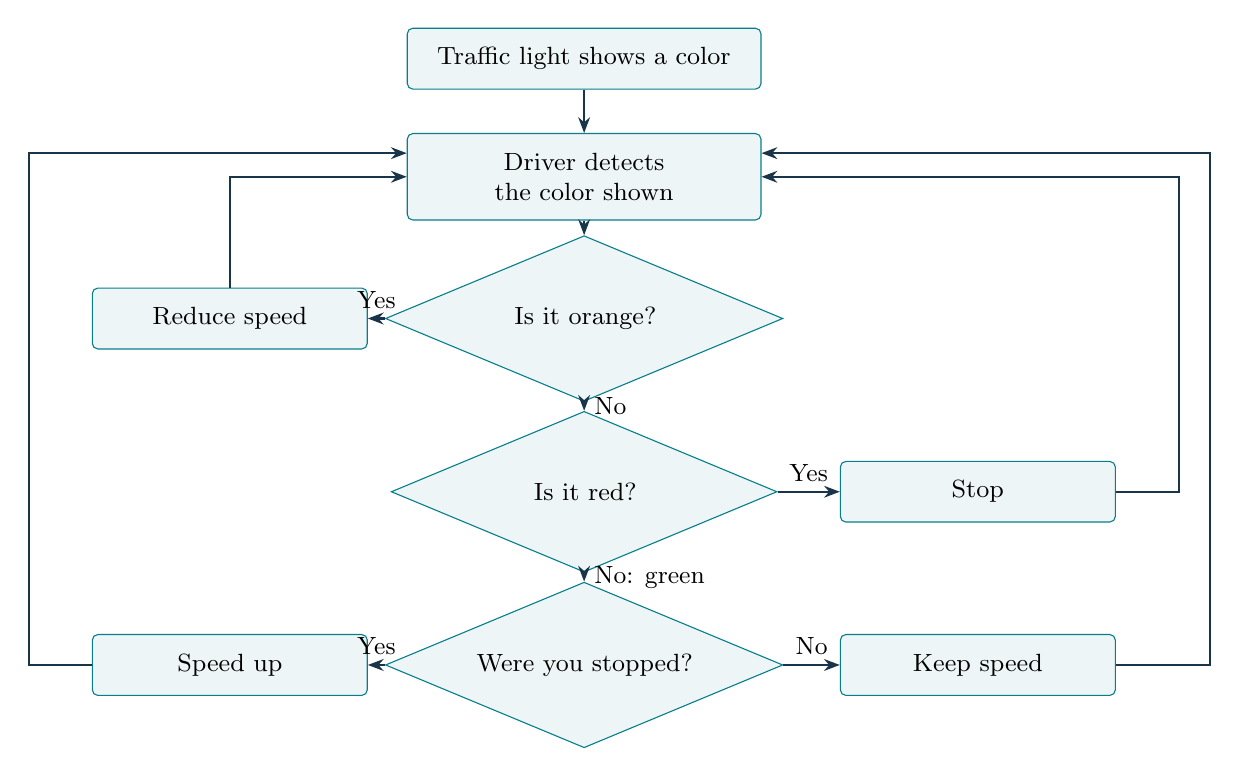
\begin{tikzpicture}
\node[box,text width=4cm] (light) at (0,0) {Traffic light shows a color};
\node[box,text width=4cm] (detect) at (0,-1.5) {Driver detects the color shown};
\node[box,diamond,rounded corners=0pt,aspect=2.4,text width=2.7cm] (orange) at (0,-3.3) {Is it orange?};
\node[box,text width=3cm] (reduce) at (-4.5,-3.3) {Reduce speed};
\node[box,diamond,rounded corners=0pt,aspect=2.4,text width=2.7cm] (red) at (0,-5.5) {Is it red?};
\node[box,text width=3cm] (stop) at (5,-5.5) {Stop};
\node[box,diamond,rounded corners=0pt,aspect=2.4,text width=2.7cm] (stopped) at (0,-7.7) {Were you stopped?};
\node[box,text width=3cm] (speedup) at (-4.5,-7.7) {Speed up};
\node[box,text width=3cm] (keep) at (5,-7.7) {Keep speed};
\draw[arr] (light)--(detect);
\draw[arr] (detect)--(orange);
\draw[arr] (orange)--node[above,font=\small]{Yes}(reduce);
\draw[arr] (reduce.north)|-(detect.west);
\draw[arr] (orange)--node[right,font=\small]{No}(red);
\draw[arr] (red)--node[above,font=\small]{Yes}(stop);
\draw[arr] (red)--node[right,font=\small]{No: green}(stopped);
\draw[arr] (stopped)--node[above,font=\small]{Yes}(speedup);
\draw[arr] (stopped)--node[above,font=\small]{No}(keep);
\draw[arr] (speedup.west)--++(.0,0)--++(-.8,0)|-([yshift=3mm]detect.west);
\draw[arr] (stop.east)--++(.8,0)|-(detect.east);
\draw[arr] (keep.east)--++(1.2,0)|-([yshift=3mm]detect.east);
\end{tikzpicture}
\end{center}
{\small\textbf{Flowchart A. Test orange first.} Orange leads to reducing speed and observing again. Otherwise, test red: stop if yes. If no, the signal is green: a stopped driver speeds up; a moving driver keeps speed. The repeated observation uses the color currently shown.}

One detection box, three decisions, and clear return paths keep the flowchart easy to follow. Returning to the same box makes repetition explicit without duplicating the operation: each visit means detecting the color again.

The stopped test reads the driver's current speed: zero means stopped. On green, speeding up gives a stopped driver a positive speed; a driver already moving retains its current speed.

Trace each color through the questions, including green for a stopped driver and for a moving driver. The \texttt{seeColor()} method updates the driver's perceived color; \texttt{adjustSpeed()} follows the appropriate response branch. On the next pass, the driver reads the color currently shown, rather than reusing the previous observation.

\subsection{Step 3: Assemble the methods into one cycle}

The return arrows mean that observation repeats on the next cycle. Execute one observation and response per driver per cycle, allowing the light to change between cycles. For this exercise, choose the following schedule:

\begin{enumerate}
\item Check whether the light's phase is due to change; call \texttt{changeColor()} when required.
\item For each driver, call \texttt{seeColor()} and then \texttt{adjustSpeed()}.
\item Record the states needed to check the cycle.
\item Advance elapsed time by one step and repeat until the stopping condition holds.
\end{enumerate}

Trace the consequence of this ordering: drivers observe the light's updated color. If observations precede the signal update, they use the previous color. Choose the order deliberately and preserve it in the implementation.


This introduces \textbf{CLOCK}: the model's organization of time and activation. Complete the cycle by answering these questions:
\begin{description}[style=nextline,leftmargin=0pt,itemsep=4pt]
\item[Iteration and time] What does one step represent, and which operations repeat?
\item[Activation and scheduling] Which elements act during the step, and in what order?
\item[Serialization or simultaneous updates] Do elements read changes made earlier in the same step, or do all read a common starting state and store changes for later application?
\item[Synchronization] If changes are stored, when are they applied together?
\item[Termination] Does the run end after a specified number of steps, at an event, or under another explicit condition?
\end{description}

For the first exercise, use a fixed run length and a declared driver order. Later, if drivers respond to one another, test whether changing that order affects the results. Simultaneous updating requires an explicit read--calculate--apply procedure; executing agents one after another does not create it automatically.

\begin{fitdisplay}
\boxed{A_4:\ \text{HOW THINGS ARE ARRANGED}\qquad FC:\ \text{HOW THINGS HAPPEN}}
\end{fitdisplay}

If practice can change a connection, an institutional prescription, or an agent's expectations, add the corresponding update at its place in the cycle. State its conditions. Where practice maintains the existing arrangement, no forced change is needed.

\clearpage


\section{Ex Post: Writing the Model Document}

The ex-post document answers:
\begin{fitdisplay}
\boxed{\textbf{What did we build, what did we do with it,}\atop\textbf{and what can we defensibly claim from it?}}
\end{fitdisplay}

Write a document with the six parts below. Use the ontology and flowcharts developed during construction, but update them to describe the model version actually assessed. Include tables, diagrams, results, and references where they make the specification and evidence explicit. This organization is a course documentation guide.

All ABMs require an auditable account. A P-ABM additionally requires evidence and a decision context supporting its proposed use. Documentation can begin during construction; the ex-post task is to reconcile the account with what was built and investigated.

\subsection{Part 1: Purpose, Question, and Scope}

Open with the phenomenon and the question the model investigates. State whether the purpose is generative exploration, support for an intervention decision, or both. Identify the population, setting, and time horizon to which the inquiry applies.

Write the question precisely enough that the reader can recognize an answer. Name the outcomes of interest and explain why they matter. State what lies outside the model's scope. For P-ABM, identify the intended decision-maker and the intervention alternatives from the beginning.

\textbf{Include:} a purpose statement, the modeling question, the scope, and definitions of the outcomes to be examined.

\subsection{Part 2: Model Specification}

Describe the model that produced the reported results. Begin with its version identifier and present the LUL diagram and flowcharts that correspond to that version.

\begin{description}[style=nextline,leftmargin=0pt,itemsep=5pt]
\item[Elements and states] Identify the represented Agents, Arena, and material and social Artificiality. Define their state variables, possible values, units where relevant, and which attributes remain fixed.
\item[Connections] Show the Array. Individual links may remain unlabeled, but explain which methods use each pathway and which states they read or affect. Specify joint conditions when a method depends on several connected elements. Distinguish location from situated agency.
\item[Methods and processes] Explain each method's inputs, conditions, decisions, and updates. Supply formulas or precise rules where a verbal description leaves more than one interpretation.
\item[Initialization and time] State how elements and connections are created, how initial values are assigned, and how activation, scheduling, time steps, and termination work. Identify any processes that reproduce or transform elements or relations during a run.
\end{description}

\textbf{Include:} the diagrams, a state-variable table, method descriptions, and initialization and scheduling rules. Reference the corresponding implementation files so the reader can follow the specification into the executable model.

For the traffic fragment, ``reduce speed'' names an operation but does not fully specify it. The document must state how much speed is reduced, when the update occurs, and how negative speed is prevented. Similarly, specify the positive speed assigned when a stopped driver resumes. These details complete the documented mechanism without adding boxes merely to describe programming syntax.

\subsection{Part 3: Assumptions and Supporting Evidence}

Make the grounds for the specification visible. Distinguish choices supported by readings or observations from course conventions, simplifying assumptions, and quantities chosen for exploration.

For each consequential assumption, record:
\begin{itemize}
\item what is assumed and where it enters the model;
\item why it is needed for the question;
\item its source or rationale;
\item the uncertainty or plausible alternatives that remain.
\end{itemize}

\textbf{Include:} an assumption-and-evidence table. For empirical inputs, document provenance, measurement, transformations, and parameter estimation. Separate evidence used to construct or calibrate the model from evidence used to assess its adequacy. If the same evidence serves both purposes, disclose that limitation.

For example, automatic compliance in the traffic exercise is a declared simplification. A policy claim about enforcement would require justification for the represented compliance behavior and an assessment of plausible alternatives.

\subsection{Part 4: Computational Experiments}

Describe what was done with the specified model. Give each experiment an identifier and a question. Record the baseline, varied settings, initial conditions, run length, output measures, and observation times. For stochastic experiments, report the replication count and seed procedure.

\textbf{Include:} an experiment table with one row per design or configuration, plus references to the run settings, outputs, and analysis files. Record software versions and dependencies needed to rerun the work. Explain how to recover the reported tables and figures from the saved outputs.

Use the following distinctions when writing the experiment table:
\begin{description}[style=nextline,leftmargin=0pt,itemsep=5pt]
\item[Replications] Repeat a specification and settings to characterize stochastic variation. State how randomness varies between runs. Repeating an identical deterministic run does not characterize uncertainty.
\item[Parameter sweeps] List the values or ranges explored and how combinations were selected. State how many replications were used at each setting.
\item[Scenarios] Define each intervention and its accompanying conditions. Identify what changes relative to the baseline: prescriptions, artifacts, access, authority, initial conditions, or process rules. Distinguish an intervention within a fixed specification from a revision of the model itself.
\end{description}

If using notation, define it alongside the experiment:
\begin{fitdisplay}
M+I_0+\theta_j+\omega_r\rightarrow T_{jr}.
\end{fitdisplay}
Here $M$ is the model specification, $I_0$ the initial conditions, $\theta_j$ the parameter setting, $\omega_r$ the stochastic realization, and $T_{jr}$ the resulting trajectory. Record any variation in initial conditions explicitly. The settings and replication count describe the evidence actually generated, not every possible behavior of the model.

\subsection{Part 5: Results and Assessment}

Present results in the order of the experiment questions. For each table or figure, identify the model version, experiment, settings, measure, units, and aggregation used. Report variation across runs where relevant. Distinguish observations from individual trajectories from patterns supported across experiments.

Then report the checks and analyses supporting interpretation:
\begin{description}[style=nextline,leftmargin=0pt,itemsep=5pt]
\item[Verification: was the specification implemented correctly?] Describe the checks performed and their results. Show that methods use the intended pathways, conditions, and state updates, and that scheduling follows the flowchart. Report unresolved discrepancies.
\item[Validation: is the model adequate for its purpose and domain?] Identify the evidence and criteria used for comparison, where the model agrees or disagrees, and what those comparisons establish. State limitations when independent evidence is unavailable.
\item[Sensitivity: what influences the results?] Report how outcomes respond to changes in parameters, initial conditions, or assumptions. Identify consequential dependencies.
\item[Robustness: which findings persist?] State which conclusions survive plausible alternative specifications or uncertainties and which do not.
\item[Cross-scenario comparison: what differs between alternatives?] Compare scenarios using common measures and explain the differences supported by the sampled trajectories. Report distributional effects and unintended consequences when relevant to the question.
\end{description}

\textbf{Include:} the result tables and figures, verification and validation evidence, and the sensitivity, robustness, and scenario comparisons performed. Where relevant, examine thresholds, regime changes, path dependence, extreme outcomes, and conditions of success or failure. State which analyses were not performed and how that limits interpretation.

\begin{principle}{Meta-analysis of simulation evidence}
In this course, \textbf{meta-analysis of simulation evidence} means assessing the model and the body of evidence produced across its computational experiments. It is broader than statistical meta-analysis of independent empirical studies. In the document, name the actual analyses and report their findings; the umbrella term does not replace them. Exploratory ABMs can benefit from these assessments, while P-ABMs must connect the assessment to their prospective claims.
\end{principle}

\subsection{Part 6: Claims, Limitations, and Decision Implications}

Answer the question stated in Part 1. Connect each main claim to the results and checks supporting it. State the assumptions, domain, and uncertainties that bound it. A selected run or convenient scenario cannot establish a general policy effect.

\textbf{Include:} a claim--evidence--limitation table or an equivalent explicit account. Separate what the model generated, what the assessment supports, and what remains conjectural. Identify further evidence needed before extending the claim.

\subsubsection{For P-ABM: write conditional prospective claims}

A prospective claim need not be a point prediction. Write the conditions under which an intervention changes the distribution or structure of possible outcomes. For example:
\begin{quote}
\textbf{Under the stated assumptions and conditions, intervention $P$ changes the distribution of outcome $Y$ in the following ways, compared with the baseline.}
\end{quote}
Follow that statement with the estimated differences, uncertainty, and robustness evidence from the actual study. Do not fill the statement with an effect the experiments have not established.

\subsubsection{For P-ABM: document the decision context}

To support actionability, report:
\begin{itemize}
\item \textbf{Who can act:} the decision-maker, their authority, and what they control.
\item \textbf{What can be done:} feasible alternatives, the baseline, and resource or implementation constraints.
\item \textbf{What matters:} objectives, trade-offs, and how benefits and burdens differ across groups.
\item \textbf{Where the advice holds:} the applicable setting and horizon, remaining uncertainties, and vulnerabilities or failure conditions.
\end{itemize}

Simulation informs these judgments; it does not determine whose objectives should prevail. Explain how the evidence bears on the decision and where additional judgment is needed.

\begin{soccer}{what the policy document must report}
For a study comparing review procedures, document each procedure, the baseline, and the measures of incorrect calls, interruptions, and effects across teams. Report the comparisons and their uncertainty. Then identify staffing and technology requirements and the trade-off between accuracy and interruption. This is a reporting example, not an asserted policy effect.
\end{soccer}

\subsection{Check the Completed Document}

Use four audit questions before submitting the document:
\begin{description}[style=nextline,leftmargin=0pt,itemsep=4pt]
\item[Transparency] Can the reader identify the assumptions, elements, connections, processes, and experimental choices?
\item[Traceability] Can each claim be followed back through results and experiments to the implementation and ontology?
\item[Replicability] Can the specified experiment be rerun and its reported behavior recovered within the appropriate stochastic tolerance?
\item[Reproducibility] Are the model, data, procedures, and analytical operations sufficiently explicit and available for independent computational scrutiny?
\end{description}
These are course operational definitions; usage of replicability and reproducibility varies across disciplines. For P-ABM, also check that the document connects its evidence to feasible alternatives and a specified decision context. Auditability applies to every ABM; actionability adds requirements for policy use.

\clearpage
\section*{References and source boundaries}
\addcontentsline{toc}{section}{References and source boundaries}
The entries below document the works explicitly cited in this guide, including the earlier readings named in the opening and the foundations summarized in Section~\ref{sec:previous-foundations}. This bibliography is not the roster of the six new readings for this session, nor a complete bibliography of prior course readings. Giddens and Ostrom are discussed through Knoeri et al. and Ghorbani et al.; Lakatos is discussed through Cioffi-Revilla. This document does not claim independent consultation of their original books. Axelrod supports the discussion of simplicity and intuition; Polhill et al. provide supplementary methodological support for the distinction between intractability and undecidability.

\begingroup\small
\begin{thebibliography}{99}
\bibitem{weaver} Weaver, W. (1948). Science and complexity. \emph{American Scientist}, 36(4), 536--544.
\bibitem{simon} Simon, H. A. (1962). The architecture of complexity. \emph{Proceedings of the American Philosophical Society}, 106(6), 467--482.
\bibitem{epstein} Epstein, J. M. (1999). Agent-based computational models and generative social science. \emph{Complexity}, 4(5), 41--60.
\bibitem{cioffi} Cioffi-Revilla, C. (2010). A methodology for complex social simulations. \emph{Journal of Artificial Societies and Social Simulation}, 13(1), 7. \url{https://jasss.soc.surrey.ac.uk/13/1/7.html}
\bibitem{knoeri} Knoeri, C., Binder, C. R., \& Althaus, H.-J. (2011). An agent operationalization approach for context specific agent-based modeling. \emph{Journal of Artificial Societies and Social Simulation}, 14(2), 4. \url{https://jasss.soc.surrey.ac.uk/14/2/4.html}
\bibitem{ghorbani} Ghorbani, A., Bots, P., Dignum, V., \& Dijkema, G. (2013). MAIA: A framework for developing agent-based social simulations. \emph{Journal of Artificial Societies and Social Simulation}, 16(2), 9. \url{https://jasss.soc.surrey.ac.uk/16/2/9.html}

\bibitem{simon_behavioral_1955} Simon, H. A. (1955). A behavioral model of rational choice. \emph{The Quarterly Journal of Economics}, 69(1). \url{https://doi.org/10.2307/1884852}.
\bibitem{axtell_why_2000-1} Axtell, R. (2000). \emph{Why agents? On the varied motivations for agent computing in the social sciences}. Working Paper No.~17. Washington, D.C.: The Brookings Institution.
\bibitem{macy_factors_2002} Macy, M. W., \& Willer, R. (2002). From factors to actors: Computational sociology and agent-based modeling. \emph{Annual Review of Sociology}, 28(1), 143--166. \url{https://doi.org/10.1146/annurev.soc.28.110601.141117}.
\bibitem{kollman_chapter_2006} Kollman, K., \& Page, S. E. (2006). Computational methods and models of politics. In \emph{Handbook of Computational Economics}, Vol.~2, Chapter~29, pp.~1433--1463. Elsevier. \url{https://doi.org/10.1016/S1574-0021(05)02029-0}.

\bibitem{axelrod_complexity_1997} Axelrod, R. M. (1997). \emph{The complexity of cooperation: Agent-based models of competition and collaboration}. Princeton, NJ: Princeton University Press. \url{https://doi.org/10.1515/9781400822300}.
\bibitem{axelrod_dissemination_1997} Axelrod, R. (1997). The dissemination of culture: A model with local convergence and global polarization. \emph{Journal of Conflict Resolution}, 41(2), 203--226. \url{https://doi.org/10.1177/0022002797041002001}.
\bibitem{polhill_prediction_2021} Polhill, J. G., Hare, M., Bauermann, T., Anzola, D., Palmer, E., Salt, D., \& Antosz, P. (2021). Using agent-based models for prediction in complex and wicked systems. \emph{Journal of Artificial Societies and Social Simulation}, 24(3), 2. \url{https://doi.org/10.18564/jasss.4597}
\end{thebibliography}
\endgroup

\begin{principle}{How to read the attributions}
\textbf{Reading-grounded:} organized complexity; hierarchical organization and near-decomposability; generative explanation and its limits; progressive model sequences; context-specific situated agency; institutional action and possible non-compliance; Axelrod's emphasis on simplicity and on simulation as an aid to intuition.

\textbf{Course synthesis:} bottom-up + along the way; the history statement and Simon/Giddens bridge; Four As, six relational classes, situated-agency triad, and dynamic practice notation; the parsimonious I-ABM heuristic and the distinction between $A_{3m}$ and $A_{3s}$; progressive re-specification; restricted LUL; auditability and actionability; broad meta-analysis of simulation evidence; prospective claims; and the traffic and soccer teaching illustrations.
\end{principle}
\end{document}
